
\begin{abstract}

\end{abstract}
\section{Introduction}
Internet privacy, also commonly referred to as online privacy, is a subset of data privacy and a fundamental human right. We consider privacy to revolve around control, use and disclosure of one’s personally identifiable information.
However, our increasingly technologically-driven world puts great pressure on privacy. 
This is why several actors in the space are continuesly developinng different solutions to achieve anonymous communication and thus leveraging internet privacy.


\subsection*{State of the art}
Tor is an open-source software for enabling anonymous communication. It is based on onion routing which encapsulates messages in layers of encryption and transmits them through a series of network nodes called onion routers. Tor however is susceptible to end-to-end correlation attacks conducted by an adversary who can eavesdrop the communication channels.These attacks reveal a wide range of information like the identity of the communicating peers.
Another project based on onion routing is I2P peer-to-peer network. I2P has different design choices from those of Tor:
\begin{itemize}
    \item Packet switched instead of circuit switched: routers maintain multiple tunnels per destination which increases significantly the scalability from $O(N)$ to $O(1)$ and resilience against failures.
    \item Unidirectional instead of bidirectional tunnels: which makes deanonymization harder but needs two sets of peers to be profiled since it's unidirectional.
    \item Peer profiles instead of directory authorities: I2P’s network information is stored in a DHT (information in the DHT is inherently untrusted) while Tor’s relay network is managed by a set of nine Directory Authorities.

\end{itemize}
I2P are vulnerable to eclipse attacks since no I2P router has a full view of the global network (similar to other peer-to-peer networks) and they also protect against only local adversaries (like Tor) and thus vulnerable to timing attacks.
\\~\\Mixnets are overlay networks of mix nodes that routes messages anonymously similarly to Tor.What differentiates mixnets from Tor is that mixnets are designed to provide metadata protection from global network adversaries by using cover traffic. Because mixnets add extra latency to network traffic, they are better-suited to applications that are not as sensitive to increased latency, such as messaging or email applications while applications like real-time video streaming are better suited for Tor. 
\begin{figure}[H]
    \centering
    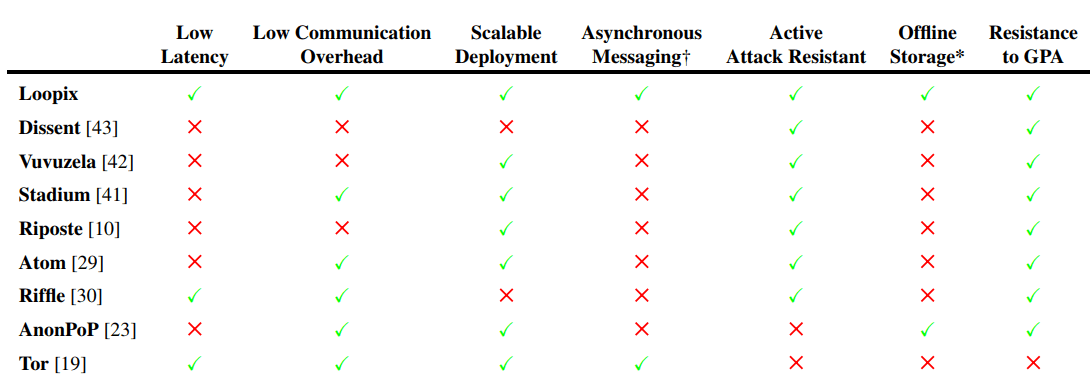
\includegraphics[width=11cm,height=11cm,keepaspectratio]{../whitepaper/images/state-of-the-art.png}
    \caption{Comparison between anonymous communication systems}
    \label{fig:Comparison between anonymous communication systems}
\end{figure}



